\section{Independent External Evaluation}
\label{sec:external-results}

AVerImaTeC changes the evidence unit, candidate store, output cap, and verdict label space. The prespecified comparisons use one locked development evaluation of five train-only seeds (Fig.~\ref{fig:external-summary}). The subsequent calibration and failure analyses reuse frozen models and outputs. The evidence diagnostics use exact normalized URLs and released image basenames. Full semantic scoring is outside the reported comparison.

\begin{figure*}[t]
    \centering
    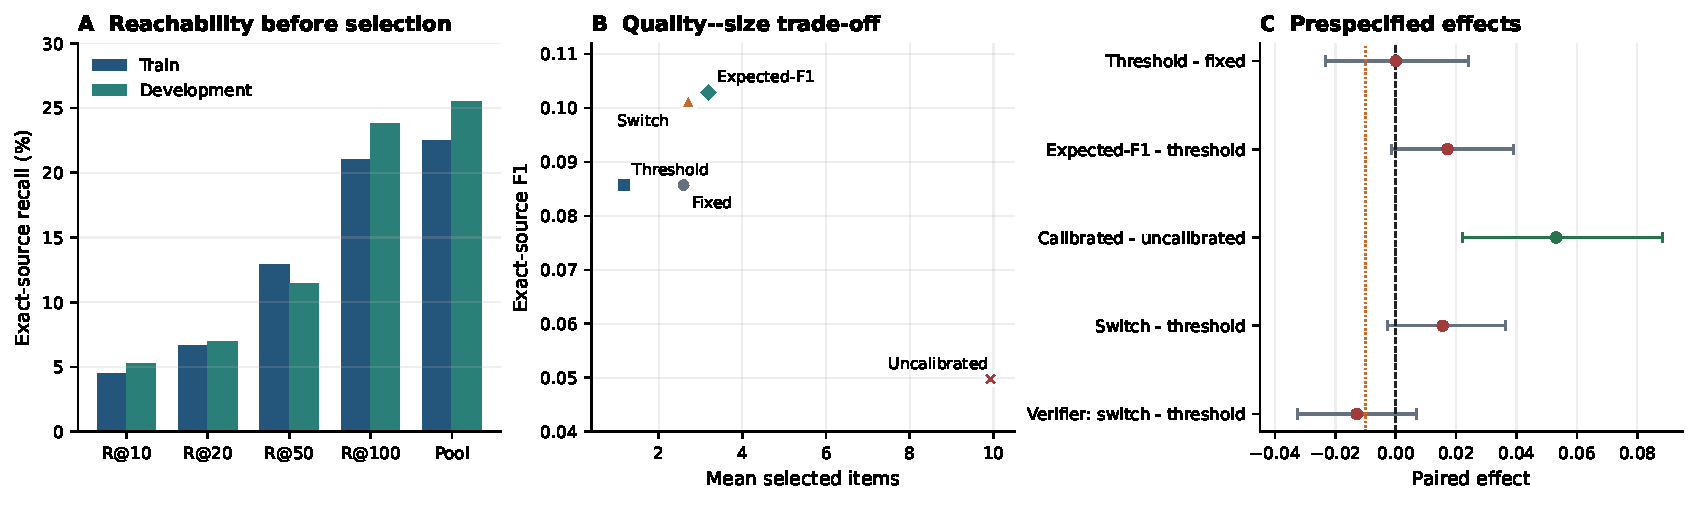
\includegraphics[width=\textwidth]{external_confirmation_summary.pdf}
    \caption{Independent AVerImaTeC development results. (a) Exact-source reachability before selection. (b) Calibrated expected-F1 has the highest diagnostic F1. Uncalibrated expected-F1 nearly reaches the ten-item cap. (c) Only the calibration effect has a positive multiplicity-adjusted interval. The verifier uses an unadjusted seed-aligned 95\% interval}
    \label{fig:external-summary}
\end{figure*}

\subsection{The Organizer Store Does Not Remove the Retrieval Ceiling}

We discovered 529,580 text and 81,817 image candidates for 793 training claims, and 101,289 text and 49,617 image candidates for 152 development claims. Each development claim has store candidates. Table~\ref{tab:external-reachability} shows how often the ranked pool contains the annotated identities.

\begin{table}[t]
\centering
\caption{Exact-source reachability before selection. Training means use 792 claims with nonempty web-source gold; development uses all 152 claims.}
\label{tab:external-reachability}
\small
\setlength{\tabcolsep}{3pt}
\begin{tabular}{@{}lrrrr@{}}
\toprule
Split & \shortstack{Pool\\recall} & Complete & Zero & \shortstack{Recall\\@100} \\
\midrule
Training & 0.2247 & 0.0922 & 0.6136 & 0.2105 \\
Development & 0.2548 & 0.1250 & 0.5987 & 0.2378 \\
\bottomrule
\end{tabular}
\end{table}

Development Recall@10, @20, and @50 is 0.0526, 0.0696, and 0.1143. The ranked pool of 100 text and 20 image candidates yields 25.48\% claim-macro recall. It contains every exact target for 19 claims and contains none for 91. This is the recall ceiling before the scorer forms a smaller packet for selection.

\subsection{Calibration on Frozen Development Candidates}

We replayed the frozen scorer and calibration map for each seed on the 18,240 ranked candidates. Table~\ref{tab:external-cal} reports candidate-weighted metrics computed per seed and averaged over seeds. The combined results pool candidate rows across modalities within each seed. Expected calibration error (ECE) uses ten equal-width probability bins, and negative log-likelihood (NLL) clips probabilities to $[10^{-12},1-10^{-12}]$. The development prevalence baseline predicts the observed positive fraction within each evaluation population and supplies a descriptive reference.

\begin{table*}[t]
\centering
\caption{Post hoc AVerImaTeC calibration on exact candidate membership. The baseline Brier score uses development prevalence. AP is average precision. Image AP is undefined because the pool contains zero exact-positive images.}
\label{tab:external-cal}
\small
\setlength{\tabcolsep}{4pt}
\begin{tabular}{llrrrrrrr}
\toprule
Candidates & Scores & Rows & Positive & Brier & Baseline Brier & NLL & ECE & AP \\
\midrule
Text & Raw & 15,200 & 86 & .18419 & .00563 & .56806 & .39639 & .06751 \\
 & Calibrated & & & .00546 & & .02948 & .00077 & .06751 \\
\addlinespace
Image & Raw & 3,040 & 0 & .00547 & 0 & .07467 & .07178 & -- \\
 & Calibrated & & & $1.44{\times}10^{-7}$ & & .00030 & .00030 & -- \\
\addlinespace
Combined & Raw & 18,240 & 86 & .15440 & .00469 & .48583 & .34229 & .06751 \\
 & Calibrated & & & .00455 & & .02461 & .00066 & .06751 \\
\bottomrule
\end{tabular}
\end{table*}

Calibration sharply reduces overconfidence and yields a combined Brier score about 3\% below the descriptive prevalence reference. AP is unchanged, consistent with an improvement in probability scale on this population. The image result reflects lower predicted probabilities on exact negatives. Positive-image probability quality remains unmeasured.

\subsection{Matched Evidence-Set Decisions}

Table~\ref{tab:external-selectors} averages within each claim over the five frozen seeds, then over claims. Calibrated expected-F1 has the highest point estimate (0.1029) at 3.20 unique identities per claim. Thresholding returns the smallest sets (1.17). Uncalibrated expected-F1 nearly fills the ten-item cap and reaches 0.0497 F1.

A modality audit found only text in the 3,800 frozen policy outputs, although the ranked pool included image candidates. The external selection comparison therefore measures policy behavior on text selections for multimodal claims. It leaves the value of selected visual evidence open.

\begin{table*}[t]
\centering
\caption{Exact-source results on locked AVerImaTeC development, averaged over five train-only seeds.}
\label{tab:external-selectors}
\small
\setlength{\tabcolsep}{7pt}
\begin{tabular}{lccccc}
\toprule
Policy & Precision & Recall & F1 & Exact set & Items \\
\midrule
Train-selected fixed top-$k$ & 0.0846 & 0.1116 & 0.0857 & 0.0053 & 2.59 \\
Calibrated threshold & \textbf{0.1308} & 0.0725 & 0.0857 & \textbf{0.0289} & \textbf{1.17} \\
Calibrated expected-F1 & 0.1198 & 0.1214 & \textbf{0.1029} & 0.0145 & 3.20 \\
Uncalibrated expected-F1 & 0.0306 & \textbf{0.1614} & 0.0497 & 0.0000 & 9.93 \\
Completeness-aware switch & 0.1208 & 0.1160 & 0.1013 & 0.0145 & 2.71 \\
\bottomrule
\end{tabular}
\end{table*}

Table~\ref{tab:external-decisions} reports 10,000 paired claim-bootstrap draws with 98.75\% per-comparison intervals for 95\% simultaneous coverage and Holm-adjusted $p$-values. Threshold superiority remains unestablished. Expected-F1 clears the $-0.010$ non-inferiority margin against thresholding and misses the compactness gate, returning about 174\% more identities. The calibration ablation clears its gate. The switch improves the point estimate in each seed, while its adjusted interval crosses zero.

\begin{table*}[t]
\centering
\caption{Prespecified external comparison family. CI denotes the simultaneous interval after Bonferroni correction.}
\label{tab:external-decisions}
\small
\setlength{\tabcolsep}{5pt}
\begin{tabular}{lrrrc}
\toprule
Comparison & Mean effect & Simultaneous CI & Holm $p$ & Gate \\
\midrule
Threshold $-$ fixed & $+0.00003$ & $[-0.02341,\,0.02404]$ & 0.9989 & \fail \\
Expected-F1 $-$ threshold & $+0.01714$ & $[-0.00148,\,0.03905]$ & 0.0714 & compactness \fail \\
Calibrated $-$ uncalibrated expected-F1 & $+0.05316$ & $[0.02207,\,0.08852]$ & 0.0008 & \pass \\
Switch $-$ threshold & $+0.01555$ & $[-0.00263,\,0.03621]$ & 0.0714 & \fail \\
\bottomrule
\end{tabular}
\end{table*}

\subsection{The Downstream Safeguard Fails Externally}

The mean verifier macro-F1 is 0.1573 (threshold evidence) and 0.1444 (switch evidence) (Table~\ref{tab:external-verifier}). The seed-aligned switch-minus-threshold effect is $-0.01293$ with 95\% interval $[-0.03242,0.00687]$ which does not exceed the reported $-0.010$. The switch therefore fails verifier non-inferiority, unlike the aggregate MOCHEG result.

\begin{table*}[t]
\centering
\caption{Five-seed mean four-class verifier results on locked development. CE/C denotes Conflicting Evidence/Cherrypicking.}
\label{tab:external-verifier}
\begin{tabular}{lrrrrrr}
\toprule
Evidence policy & Acc. & Macro-F1 & Sup. & Ref. & NEI & CE/C \\
\midrule
Threshold & 0.3158 & \textbf{0.1573} & 0.1150 & 0.4710 & 0.0432 & 0.0000 \\
Switch & 0.2842 & 0.1444 & 0.1000 & 0.4300 & 0.0474 & 0.0000 \\
\bottomrule
\end{tabular}
\end{table*}

The development split contains 141 Refuted, six Not Enough Evidence, four Supported, and one Conflicting claim. Both policies miss the Conflicting example in all five seeds. We report class-wise results and macro-F1 because accuracy alone gives little information about the rare verdicts.

\subsection{Where Exact Evidence Was Lost}

We traced 337 claim--target identities through the indexed store, usable candidate discovery, ranked pool, scorer packet, and saved selections. Each seed repeats the same store and pool, giving 1,685 target--seed instances. We counted each target once at its first failure stage (Fig.~\ref{fig:external-diagnostics}). Store presence means a normalized URL in the claim-indexed store entries or an exact image basename. A URL was usable if its record yielded a nonempty text segment. Basename absence cannot resolve visual equivalence.

Fourteen identities were absent by this definition, including all eight annotated image identities. A further 93 had a store URL but no usable candidate text, and 153 were discovered but ranked outside the retained pool. The store listed every exact identity for 145 of 152 claims, the usable candidates covered 79, and the pool covered 19. The scorer packet contained the complete set in 80 of 760 claim--seed instances (10.53\%). Under fixed selection, 52 target--seed instances fell outside that packet, 178 were omitted by the selector, and 155 were selected. These counts distinguish acquisition and ranking losses from selection opportunities.

\begin{figure*}[t]
\centering
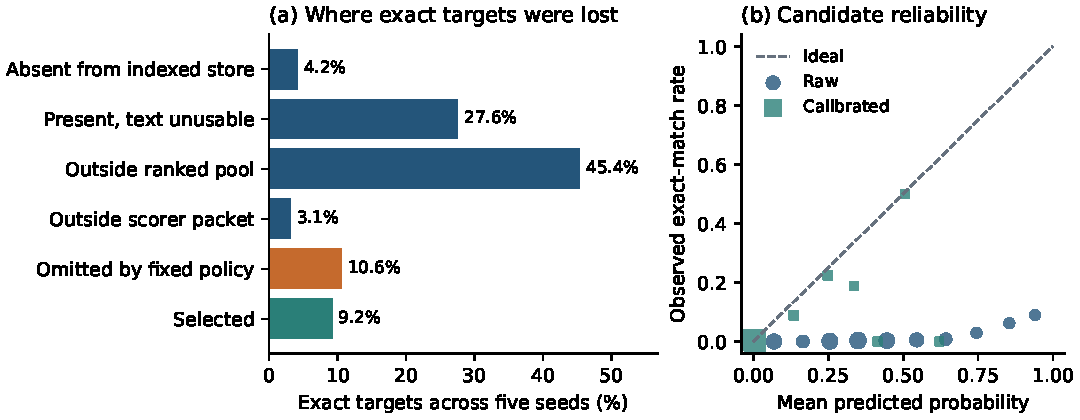
\includegraphics[width=0.93\textwidth]{one_shot_external_diagnostics.pdf}
\caption{Post hoc diagnostics on frozen AVerImaTeC development outputs. (a) Each exact target--seed instance is counted once under the fixed policy. (b) Pooled reliability across candidate rows and seeds. Point area reflects bin support, and the dashed line indicates ideal calibration}
\label{fig:external-diagnostics}
\end{figure*}

Among claim--seed instances with at least one selected exact target, the verifier made 59 errors in 103 instances under thresholding and 103 in 153 under the switch. These are claim-level associations under a shared verifier. Exact overlap can coexist with incomplete or unhelpful evidence.

\subsection{Cross-Benchmark Transfer}

Table~\ref{tab:cross-benchmark} aligns the research questions across development protocols. The metrics remain specific to each benchmark's evidence unit. Table~\ref{tab:external-disagreement} shows that the policies often return different sources even when every annotated identity is missing from the ranked pool.

\begin{table*}[t]
\centering
\caption{Development findings across benchmarks, using each benchmark's evidence units. MOCHEG and verifier intervals are paired 95\% intervals. External selector intervals use the four-comparison correction.}
\label{tab:cross-benchmark}
\small
\begin{tabular}{@{}>{\raggedright\arraybackslash}p{0.20\textwidth}*{2}{>{\raggedright\arraybackslash}p{0.365\textwidth}}@{}}
\toprule
Question & MOCHEG (1,490 claims) & AVerImaTeC (152 claims) \\
\midrule
Reachability & Text R@40 .3393 and image R@20 .3287. Complete 5.91\%, zero 13.89\%. & Pooled exact-source claim-macro recall .2548. Complete 12.50\%, zero 59.87\%. \\
Probability quality & Identity to isotonic mean Brier .0847 to .0330. Selected maps have positive Brier skill against prevalence in every partition. & Raw to frozen-map combined mean Brier .15440 to .00455, with .00469 for development prevalence. \\
Threshold vs.\ fixed & $+.01517$ $[.01114,.01923]$. & $+.00003$ $[-.02341,.02404]$. \\
Expected-F1 vs.\ threshold & $-.00484$ $[-.00938,-.00020]$ with 3.61 vs.\ 5.26 items. & $+.01714$ $[-.00148,.03905]$ with 3.20 vs.\ 1.17 identities. \\
Switch vs.\ threshold & $+.00138$ $[-.00191,.00462]$. Superiority gate fails. & $+.01555$ $[-.00263,.03621]$. Superiority gate fails. \\
Verifier preservation & $+.00434$ $[-.00277,.01130]$ macro-F1. Aggregate margin clears, seed safeguard fails. & $-.01293$ $[-.03242,.00687]$ macro-F1. Aggregate margin fails. \\
\bottomrule
\end{tabular}
\end{table*}

\begin{table}[t]
\centering
\caption{Policy disagreement by ranked-pool exact reachability. Each cell gives unequal source sets out of the indicated claim--seed denominator.}
\label{tab:external-disagreement}
\small
\setlength{\tabcolsep}{3pt}
\begin{tabular}{@{}lrrr@{}}
\toprule
Policy vs.\ threshold & Zero & Partial & Complete \\
\midrule
Fixed & 349/455 & 167/210 & 72/95 \\
Expected-F1 & 384/455 & 144/210 & 74/95 \\
Switch & 308/455 & 124/210 & 64/95 \\
\bottomrule
\end{tabular}
\end{table}

\subsection{Frozen Decision}

Under the frozen decision rule, the switch requires superiority and verifier preservation, expected-F1 requires non-inferiority and at least 15\% fewer identities than thresholding, and thresholding requires superiority over fixed selection. The rule defaulted to the train-selected fixed family. Its five local development exports meet the organizer's ten-item and 1,500-character limits. Formal test annotations remain sealed.
